%-----------------------------------------------------------------------------%
\chapter{\babLima}
\label{bab:5}

Bab ini membahas mengenai hasil dan analisis dari evaluasi yang telah dilaksanakan berdasarkan skenario-skenario yang telah disusun pada bab sebelumnya. Pembahasan analisis akan dibagikan berdasarkan aspek-aspek yang telah disusun untuk memberikan gambaran yang lebih jelas mengenai performa program dan \textit{resource} atau sumber daya yang dibutuhkan untuk mencapai performa tersebut. Selain itu, bab ini juga akan membahas pertimbangan variasi dari PeerToCP yang lebih baik digunakan dan faktor-faktor yang memengaruhi pertimbangan tersebut. Melalui pertimbangan tersebut, kelemahan dari sistem aplikasi turut disampaikan untuk perkembangan ke depannya.

\section{Aspek \textit{Local-First} dan \textit{Correctness}}

Kedua aspek ini tidak dapat dipisahkan satu sama lain, pada skenario pertama dan kedua, aspek \textit{local-first} diuji dengan mensimulasikan proses pemutusan koneksi secara acak pada klien, sementara data terus diubah oleh setiap pengguna lokal. Berdasarkan eksperimen secara langsung, proses perubahan ini terjadi secara \textit{local-first}, yang berarti perubahan lokal dapat terus dilakukan dan langsung diterapkan meskipun klien sedang tidak berada dalam jaringan, dan ketika terjadi proses masuk kembali ke jaringan, data akan diperbaharui secara sesuai dengan perubahan yang dilakukan.

Berdasarkan eksperimen yang dilakukan, setiap variasi dari PeerToCP menghasilkan nilai cacahan yang sama untuk setiap skenarionya, yang berarti setiap dokumen berada pada kondisi atau \textit{state} akhir yang sama. Namun pada skenario pertama dengan 8 klien pada variasi Operational Transformation yang berbasis \textit{Client-Server}, dapat terjadi pemutusan hubungan \textit{disconnection} yang tidak dapat terhubung kembali karena \textit{bandwidth} koneksi internet yang berada di luar batas \textit{environment} pengujian.

Skenario dengan jumlah klien ini diulang hingga tiga kali eksperimen, dan dalam setiap eksperimen tersebut, satu hingga dua klien tidak dapat terhubung kembali. Perhatikan bahwa pada eksperimen, waktu pemutusan hubungan dilakukan secara acak dalam periode durasi yang sama untuk setiap kliennya seperti yang dijelaskan pada bab sebelumnya. Hal ini ditunjukkan secara lebih detail pada grafik transmisi data yang masuk melalui jaringan pada klien pertama dan klien kedua untuk setiap variasi aplikasi dalam skenario pertama ini.

\begin{figure}
 \centering
 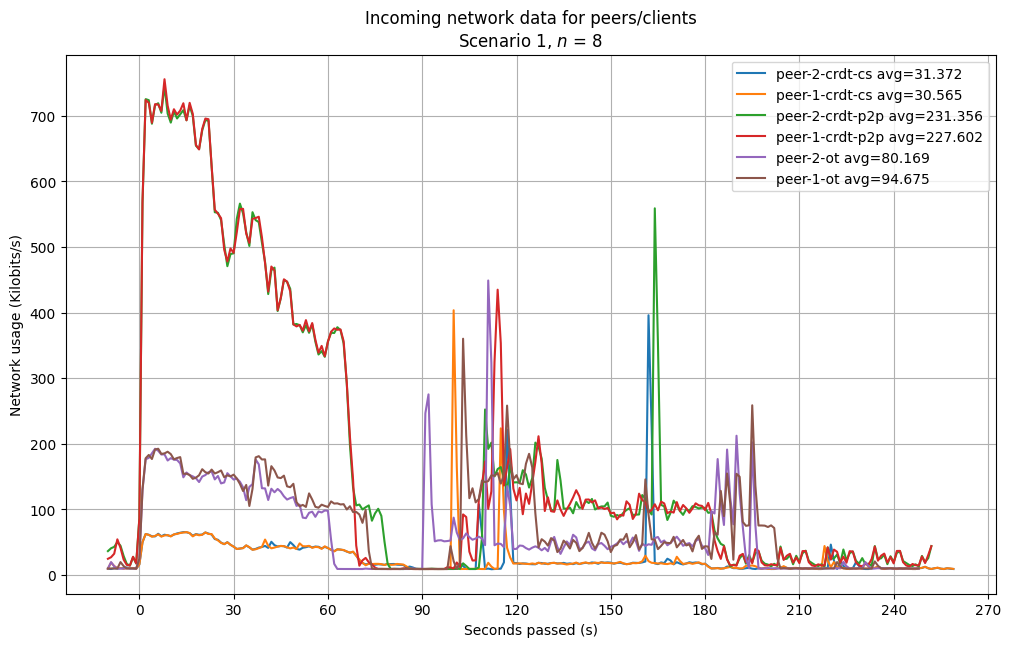
\includegraphics[width=13cm]{./assets/skripsi/benchmark-vis_cell_2_output_23}
 \caption{Grafik Perbandingan Jaringan pada Klien Pertama dan Klien Kedua untuk $n = 8$}
 \label{fig:2-23}
\end{figure}

Pada saat operasi \textit{update} dilakukan tepat setelah koneksi terhubung kembali, ukuran \textit{update} cenderung lebih besar karena sudah terkumpul dari beberapa operasi yang terjadi selama klien sedang berada di luar jaringan. Ketika \textit{update} ini dilakukan, server sedang dalam keadaan berbagai klien lain yang hendak mengirimkan \textit{update}. Karena hal tersebut, algoritma \textit{operational transformation} yang hanya membolehkan suatu \textit{update} untuk dilakukan apabila versi terbaru yang sama sudah dimiliki oleh klien akan meminta klien untuk melakukan \textit{update}. Sementara tumpukan \textit{push update} berukuran besar terus dikirimkan hal ini akan memenuhi \textit{bandwidth} server, yang dapat dilihat pada grafik berikut.

Perhatikan bahwa pada Gambar~\ref{fig:2-23}, menunjukkan klien pertama yang mengalami pemutusan jaringan pada detik ke-72 dan penghubungan kembali pada detik ke-102, terjadi pengiriman data yang cukup besar selama kurang lebih 20 detik. Begitu pula dengan klien kedua yang mengalami pemutusan jaringan pada sekitar detik ke-60 dan penghubungan kembali pada detik ke-90. Sesaat setelah suatu klien terhubung kembali ke suatu jaringan, akan terjadi \textit{spike} pada jaringan yang cukup besar. Pada jumlah pengguna yang cukup banyak dalam satu dokumen, pemutusan dan penghubungan jaringan yang secara sengaja dilakukan pada waktu yang serupa dapat menyebabkan ketidakandalan pada sistem ini. Grafik untuk server ditunjukkan pada gambar berikut.

\begin{figure}
 \centering
 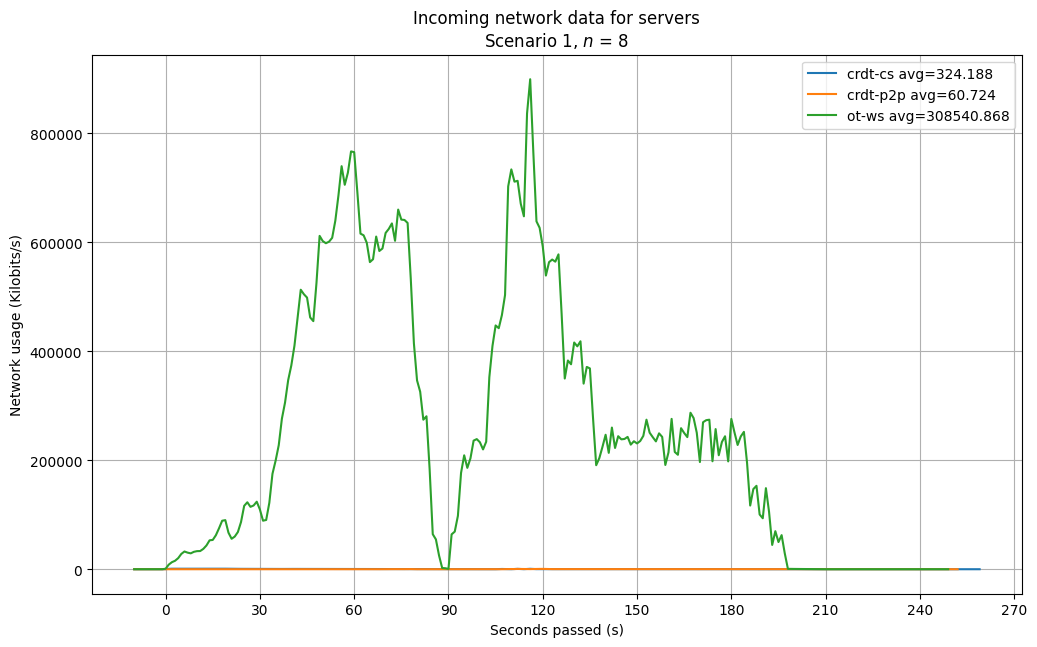
\includegraphics[width=15cm]{./assets/skripsi/benchmark-vis_cell_2_output_24}
 \caption{Grafik Perbandingan Penerimaan Data pada Setiap Variasi Server PeerToCP}
 \label{fig:2-24}
\end{figure}

Lalu lintas jaringan pada server variasi \textit{operational transformation} dengan arsitektur \textit{client-server} dapat mencapai lebih dari 800000 \textit{kilobits}/detik atau setara dengan 100 \textit{megabytes}/detik, sementara untuk skenario yang serupa, transmisi data pada server dengan variasi CRDT berarsitektur \textit{client-server} lebih hemat sekitar 950 kali. Melalui Gambar~\ref{fig:2-24}, diketahui bahwa mean transmisi jaringannya sekitar 80 kali lebih sedikit dibandingkan CRDT \textit{peer-to-peer} serta 950 kali lebih sedikit dibandingkan CRDT \textit{client-server}.

Pada skenario pertama ini, terlihat bahwa variasi PeerToCP yang menggunakan CRDT lebih dapat diandalkan karena paralelitas \textit{update} yang dilakukan terhadap dokumen. Faktor-faktor lain yang memengaruhi variasi CRDT yang lebih baik juga tidak menutup kemungkinan dari segi implementasi \textit{provider websocket} yang digunakan, teknik kompresi dan \textit{encoding} yang diterapkan, serta efek bola salju yang ditimbulkan akibat \textit{update} berukuran besar yang terus dikirimkan menjadi tertumpuk dan selalu terlambat dibandingkan \textit{update} lain dan menyangkut aspek selanjutnya yang akan dibahas, yaitu \textit{Scalability} dan \textit{Responsiveness}.

\section{Aspek \textit{Scalability} dan \textit{Responsiveness}}

Latensi dari teks editor secara khusus diukur secara terus menerus pada skenario ketiga. Setiap klien atau \textit{peer} akan diukur waktu selisih penerimaan datanya dan dicatat latensinya pada waktu data dokumen diterima, kemudian dilakukan rata-rata untuk $n$ klien-klien atau \textit{peers} tersebut tabel~\ref{tab:latency-3} menunjukkan latensi PeerToCP variasi CRDT \textit{peer-to-peer} memiliki latensi yang paling rendah, namun semakin besar nilai $n$, selisih perbedaan CRDT \textit{client-server} dan CRDT \textit{peer-to-peer} semakin mengecil. Sementara pada variasi OT \textit{client-server}, latensinya dua kali lebih besar dari variasi CRDT \textit{client-server}, dengan lonjakan latensi maksimum hingga dua detik saat $n = 8$.

% Please add the following required packages to your document preamble:
% \usepackage{multirow}
\begin{table}[H]
 \centering
 \caption{Deskripsi Statistik Latensi Skenario Ketiga dalam ms}
\begin{tabular}{|c|rrr|rrr|rrr|}
\hline
\multirow{2}{*}{$n$} & \multicolumn{3}{c|}{\textbf{CRDT Peer-To-Peer}} & \multicolumn{3}{c|}{\textbf{CRDT Client Server}} & \multicolumn{3}{c|}{\textbf{OT Client Server}} \\ \cline{2-10}
 & \multicolumn{1}{c|}{Mean} & \multicolumn{1}{c|}{Median} & \multicolumn{1}{c|}{Max} & \multicolumn{1}{c|}{Mean} & \multicolumn{1}{c|}{Median} & \multicolumn{1}{c|}{Max} & \multicolumn{1}{c|}{Mean} & \multicolumn{1}{c|}{Median} & \multicolumn{1}{c|}{Max} \\ \hline
\textbf{2} & \multicolumn{1}{r|}{23.30} & \multicolumn{1}{r|}{21.00} & 76.00 & \multicolumn{1}{r|}{39.50} & \multicolumn{1}{r|}{38.00} & 134.00 & \multicolumn{1}{r|}{87.42} & \multicolumn{1}{r|}{84.00} & 168.00 \\ \hline
\textbf{4} & \multicolumn{1}{r|}{34.00} & \multicolumn{1}{r|}{30.00} & 223.00 & \multicolumn{1}{r|}{46.10} & \multicolumn{1}{r|}{42.00} & 220.00 & \multicolumn{1}{r|}{98.84} & \multicolumn{1}{r|}{86.00} & 1225.00 \\ \hline
\textbf{8} & \multicolumn{1}{r|}{55.56} & \multicolumn{1}{r|}{47.00} & 313.00 & \multicolumn{1}{r|}{63.84} & \multicolumn{1}{r|}{56.00} & 308.00 & \multicolumn{1}{r|}{235.62} & \multicolumn{1}{r|}{151.00} & 2010.00 \\ \hline
\end{tabular}
 \label{tab:latency-3}
\end{table}

Dari segi skalabilitasnya, dengan asumsi pengguna berada dalam jarak yang dekat, misalnya dalam kasus ini setiap \textit{peers} berada dalam satu zona yang sama, yaitu Indonesia. Variasi \textit{peer-to-peer} memberikan performa yang optimal dibandingkan \textit{client-server} untuk jumlah $n$ tertentu. Berdasarkan perhitungan dan proyeksi jumlah pengguna yang bertambah, variasi dari CRDT \textit{client-server} dapat memberikan \textit{responsiveness} yang lebih baik untuk suatu nilai $n$ yang lebih tinggi atau saat \textit{peers} berada pada daerah yang lebih jauh antara satu sama lainnya.

\begin{table}[H]
 \centering

 \caption{Deskripsi Statistik Aktivitas dan \textit{Resource Server} pada Skenario Pertama}
\begin{tabular}{|cc|r|r|r|}
\hline
\multicolumn{2}{|c|}{$\boldsymbol{n}$} & \multicolumn{1}{c|}{\textbf{2}} & \multicolumn{1}{c|}{\textbf{4}} & \multicolumn{1}{c|}{\textbf{8}} \\ \hline
\multicolumn{1}{|c|}{\multirow{4}{*}{\textbf{CRDT Peer-To-Peer}}} & CPU & 0.01 & 0.02 & 0.10 \\ \cline{2-5}
\multicolumn{1}{|c|}{} & RAM & 0.67 & -0.03 & 0.40 \\ \cline{2-5}
\multicolumn{1}{|c|}{} & Net In & 10.72 & 14.81 & 60.72 \\ \cline{2-5}
\multicolumn{1}{|c|}{} & Net Out & -10.24 & -15.79 & -83.11 \\ \hline
\multicolumn{1}{|c|}{\multirow{4}{*}{\textbf{CRDT Client Server}}} & CPU & 0.93 & 1.29 & 1.68 \\ \cline{2-5}
\multicolumn{1}{|c|}{} & RAM & 5.01 & 6.83 & 9.54 \\ \cline{2-5}
\multicolumn{1}{|c|}{} & Net In & 73.26 & 176.64 & 324.19 \\ \cline{2-5}
\multicolumn{1}{|c|}{} & Net Out & -71.79 & -193.90 & -391.66 \\ \hline
\multicolumn{1}{|c|}{\multirow{4}{*}{\textbf{OT Client Server}}} & CPU & 4.85 & 14.18 & 24.33 \\ \cline{2-5}
\multicolumn{1}{|c|}{} & RAM & 30.92 & 41.88 & 69.99 \\ \cline{2-5}
\multicolumn{1}{|c|}{} & Net In & 52318.08 & 167768.04 & 308540.87 \\ \cline{2-5}
\multicolumn{1}{|c|}{} & Net Out & -26494.76 & -84932.31 & -156178.28 \\ \hline
\end{tabular}
\end{table}

\begin{table}[H]
 \centering
 \caption{Deskripsi Statistik Aktivitas dan \textit{Resource} Klien atau \textit{Peers} pada Skenario Pertama}

\begin{tabular}{|cc|r|r|r|}
\hline
\multicolumn{2}{|c|}{$n$} & \multicolumn{1}{c|}{\textbf{2}} & \multicolumn{1}{c|}{\textbf{4}} & \multicolumn{1}{c|}{\textbf{8}} \\ \hline
\multicolumn{1}{|c|}{\multirow{4}{*}{\textbf{CRDT Peer-To-Peer}}} & CPU & 39.1964893 & 60.13947488 & 62.2870496 \\ \cline{2-5}
\multicolumn{1}{|c|}{} & RAM & 16.57856816 & 19.24442935 & 21.30499303 \\ \cline{2-5}
\multicolumn{1}{|c|}{} & Net In & 28.5230253 & 96.16536701 & 229.4788353 \\ \cline{2-5}
\multicolumn{1}{|c|}{} & Net Out & -28.03809012 & -93.97903876 & -223.6266535 \\ \hline
\multicolumn{1}{|c|}{\multirow{4}{*}{\textbf{CRDT Client Server}}} & CPU & 33.96390498 & 57.38616741 & 56.89049428 \\ \cline{2-5}
\multicolumn{1}{|c|}{} & RAM & 14.92823532 & 19.12934751 & 20.94699478 \\ \cline{2-5}
\multicolumn{1}{|c|}{} & Net In & 19.46582482 & 27.68880062 & 30.96869733 \\ \cline{2-5}
\multicolumn{1}{|c|}{} & Net Out & -19.76281471 & -21.21326889 & -18.73440885 \\ \hline
\multicolumn{1}{|c|}{\multirow{4}{*}{\textbf{OT Client Server}}} & CPU & 47.79374975 & 73.29454876 & 65.25737338 \\ \cline{2-5}
\multicolumn{1}{|c|}{} & RAM & 25.9460194 & 31.17265199 & 36.33549154 \\ \cline{2-5}
\multicolumn{1}{|c|}{} & Net In & 62.24127487 & 99.81376692 & 87.42216719 \\ \cline{2-5}
\multicolumn{1}{|c|}{} & Net Out & -12962.04576 & -28872.47276 & -18344.14905 \\ \hline
\end{tabular}
\end{table}

\section{Evaluasi Latensi}


% Please add the following required packages to your document preamble:
% \usepackage{multirow}
\begin{table}[H]
 \centering
 \caption{Deskripsi Statistik Latensi Skenario Keempat dalam ms}
\begin{tabular}{|c|rrr|rrr|rrr|}
\hline
\multirow{2}{*}{$n$} & \multicolumn{3}{c|}{\textbf{CRDT Peer-To-Peer}} & \multicolumn{3}{c|}{\textbf{CRDT Client Server}} & \multicolumn{3}{c|}{\textbf{OT Client Server}} \\ \cline{2-10}
 & \multicolumn{1}{c|}{Mean} & \multicolumn{1}{c|}{Median} & \multicolumn{1}{c|}{Max} & \multicolumn{1}{c|}{Mean} & \multicolumn{1}{c|}{Median} & \multicolumn{1}{c|}{Max} & \multicolumn{1}{c|}{Mean} & \multicolumn{1}{c|}{Median} & \multicolumn{1}{c|}{Max} \\ \hline
\textbf{2} & \multicolumn{1}{r|}{3.05} & \multicolumn{1}{r|}{3.00} & 5.00 & \multicolumn{1}{r|}{16.75} & \multicolumn{1}{r|}{17.00} & 19.00 & \multicolumn{1}{r|}{31.79} & \multicolumn{1}{r|}{30.00} & 170.00 \\ \hline
\textbf{4} & \multicolumn{1}{r|}{3.13} & \multicolumn{1}{r|}{3.00} & 6.00 & \multicolumn{1}{r|}{16.55} & \multicolumn{1}{r|}{17.00} & 21.00 & \multicolumn{1}{r|}{44.47} & \multicolumn{1}{r|}{32.00} & 309.00 \\ \hline
\textbf{8} & \multicolumn{1}{r|}{3.36} & \multicolumn{1}{r|}{3.00} & 19.00 & \multicolumn{1}{r|}{17.16} & \multicolumn{1}{r|}{17.00} & 35.00 & \multicolumn{1}{r|}{59.86} & \multicolumn{1}{r|}{30.33} & 551.00 \\ \hline
\end{tabular}
\end{table}



\section{Evaluasi Performa}